\documentclass{article}
\usepackage[utf8]{inputenc}
\usepackage[spanish]{babel}
\usepackage{graphicx}
\title{Modelos matemáticos discretos}
\author{Eduardo Perez Olvera}
\begin{document}
\maketitle
\section{Ecuaciones en diferencias}
\subsection{Primer orden}
Tenemos \$1000 que vamos a invertir a un interés de 1\% mensual.

El valor de la inversión cuando han transcurrido $n$ meses es $$x_n=1000(1.01)^n$$.
Una gráfica del resultado es:

\begin{center}
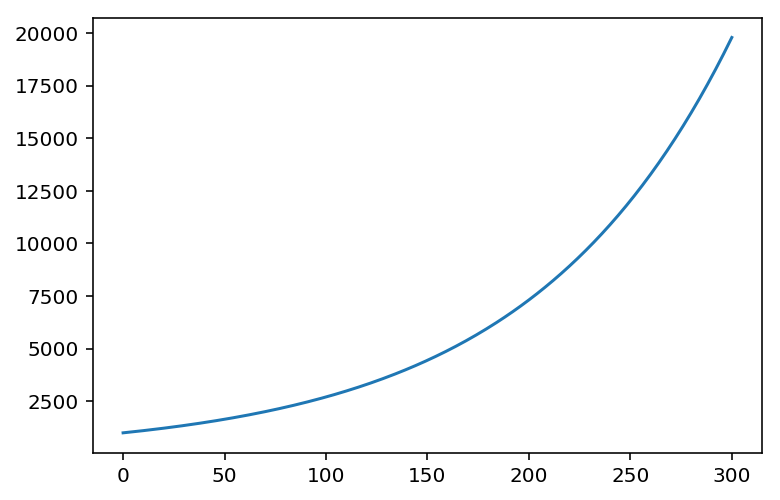
\includegraphics[width=8cm]{a}
\end{center}

\begin{center}\begin{tabular}{|c|c|}
\hline
interante & valor \\
\hline
0 & 1000 \\
\hline
1 & 1010 \\
\hline
2 & 1021.10 \\
\hline
3 & 1030.301\\
\hline
\end{tabular}\end{center}

Para encontrar este resultado, ocupamos que
$$\sum_{i=0}^{n-1}a^i=\frac{1-a^{n}}{1-a}$$
\subsection{Segundo orden}
\end{document}
